%%%%%%%%%%%%%%%%%%%%%%%%%%%%%%%%%%%%%%%%%
% Masters/Doctoral Thesis 
% LaTeX Template
% Version 2.5 (27/8/17)
%
% This template was downloaded from:
% http://www.LaTeXTemplates.com
%
% Version 2.x major modifications by:
% Vel (vel@latextemplates.com)
%
% This template is based on a template by:
% Steve Gunn (http://users.ecs.soton.ac.uk/srg/softwaretools/document/templates/)
% Sunil Patel (http://www.sunilpatel.co.uk/thesis-template/)
%
% Template license:
% CC BY-NC-SA 3.0 (http://creativecommons.org/licenses/by-nc-sa/3.0/)
%
%%%%%%%%%%%%%%%%%%%%%%%%%%%%%%%%%%%%%%%%%

%----------------------------------------------------------------------------------------
%	PACKAGES AND OTHER DOCUMENT CONFIGURATIONS
%----------------------------------------------------------------------------------------

\documentclass[
11pt, % The default document font size, options: 10pt, 11pt, 12pt
oneside, % Two side (alternating margins) for binding by default, uncomment to switch to one side
english, % ngerman for German
singlespacing, % Single line spacing, alternatives: onehalfspacing or 
%doublespacing,
%draft, % Uncomment to enable draft mode (no pictures, no links, overfull hboxes indicated)
%nolistspacing, % If the document is onehalfspacing or doublespacing, uncomment this to set spacing in lists to single
liststotoc, % Uncomment to add the list of figures/tables/etc to the table of contents
%toctotoc, % Uncomment to add the main table of contents to the table of contents
parskip, % Uncomment to add space between paragraphs
%nohyperref, % Uncomment to not load the hyperref package
%headsepline, % Uncomment to get a line under the header
%chapterinoneline, % Uncomment to place the chapter title next to the number on one line
%consistentlayout, % Uncomment to change the layout of the declaration, abstract and acknowledgements pages to match the default layout
]{MastersDoctoralThesis} % The class file specifying the document structure

\usepackage[utf8]{inputenc} % Required for inputting international characters
\usepackage[T1]{fontenc} % Output font encoding for international characters

\usepackage{mathpazo} % Use the Palatino font by default
%\usepackage[backend=bibtex,style=authoryear,natbib=true]{biblatex} % Use the bibtex backend with the authoryear citation style (which resembles APA)


\usepackage[autostyle=true]{csquotes} % Required to generate language-dependent quotes in the bibliography
\usepackage[backend=biber,style=alphabetic,sorting=ynt]{biblatex}
\addbibresource{example.bib} % The filename of the bibliography

%----------------------------------------------------------------------------------------
%	MARGIN SETTINGS
%----------------------------------------------------------------------------------------

\geometry{
	paper=a4paper, % Change to letterpaper for US letter
	inner=2.5cm, % Inner margin
	outer=3.8cm, % Outer margin
	bindingoffset=.5cm, % Binding offset
	top=1.5cm, % Top margin
	bottom=1.5cm, % Bottom margin
	%showframe, % Uncomment to show how the type block is set on the page
}

%----------------------------------------------------------------------------------------
%	THESIS INFORMATION
%----------------------------------------------------------------------------------------

\thesistitle{A Reynolds Number Based Sampling Techniques for 3-D Vector Fields in Computational Fluid Dynamic Environments} % Your thesis title, this is used in the title and abstract, print it elsewhere with \ttitle
\supervisor{} % Your supervisor's name, this is used in the title page, print it elsewhere with \supname
\examiner{} % Your examiner's name, this is not currently used anywhere in the template, print it elsewhere with \examname
\degree{Masters of Computer Science} % Your degree name, this is used in the title page and abstract, print it elsewhere with \degreename
\author{Trent \textsc{Schweitzer}} % Your name, this is used in the title page and abstract, print it elsewhere with \authorname
\addresses{} % Your address, this is not currently used anywhere in the template, print it elsewhere with \addressname

\subject{Computer Sciences} % Your subject area, this is not currently used anywhere in the template, print it elsewhere with \subjectname
\keywords{} % Keywords for your thesis, this is not currently used anywhere in the template, print it elsewhere with \keywordnames
\university{\href{http://www.university.com}{University of Montana}} % Your university's name and URL, this is used in the title page and abstract, print it elsewhere with \univname
\department{\href{http://department.university.com}{Department of Computer Science} }% Your department's name and URL, this is used in the title page and abstract, print it elsewhere with \deptname
%\group{\href{http://researchgroup.university.com}{Research Group Name}} % Your research group's name and URL, this is used in the title page, print it elsewhere with \groupname
\faculty{\href{http://faculty.university.com}{Faculty Name}} % Your faculty's name and URL, this is used in the title page and abstract, print it elsewhere with \facname

\AtBeginDocument{
\hypersetup{pdftitle=\ttitle} % Set the PDF's title to your title
\hypersetup{pdfauthor=\authorname} % Set the PDF's author to your name
\hypersetup{pdfkeywords=\keywordnames} % Set the PDF's keywords to your keywords
}

\begin{document}

\frontmatter % Use roman page numbering style (i, ii, iii, iv...) for the pre-content pages

\pagestyle{plain} % Default to the plain heading style until the thesis style is called for the body content

%----------------------------------------------------------------------------------------
%	TITLE PAGE
%----------------------------------------------------------------------------------------

\begin{titlepage}
\begin{center}

\vspace*{.06\textheight}
{\scshape\LARGE \univname\par}\vspace{1.5cm} % University name
\textsc{\Large Masters Thesis}\\[0.5cm] % Thesis type

\HRule \\[0.4cm] % Horizontal line
{\huge \bfseries \ttitle\par}\vspace{0.4cm} % Thesis title
\HRule \\[1.5cm] % Horizontal line
 
\begin{minipage}[t]{0.4\textwidth}
\begin{flushleft} \large
\emph{Author:}\\
{\authorname} % Author name - remove the \href bracket to remove the link
\end{flushleft}
\end{minipage}
% \begin{minipage}[t]{0.4\textwidth}
% \begin{flushright} \large
% \emph{Supervisor:} \\
% \href{http://www.jamessmith.com}{\supname} % Supervisor name - remove the \href bracket to remove the link  
% \end{flushright}
% \end{minipage}\\[3cm]
 
\vfill

\large \textit{A thesis submitted in fulfillment of the requirements\\ for the degree of \degreename}\\[0.3cm] % University requirement text
\textit{in the}\\[0.4cm]
\deptname\\[2cm] % Research group name and department name
 
\vfill

{\large \today}\\[4cm] % Date
%\includegraphics{Logo} % University/department logo - uncomment to place it
 
\vfill
\end{center}
\end{titlepage}





%----------------------------------------------------------------------------------------
%	ABSTRACT PAGE
%----------------------------------------------------------------------------------------

\begin{abstract}
\addchaptertocentry{\abstractname} % Add the abstract to the table of contents
Effective visualization of unsteady,time-dependent, vector fields in a virtual environment is not a trivial task. This is due to most visualization techniques requiring the user to have a preemptive understanding of how the wind will behave before the simulation can be visualized. In this paper we will take air data flow from Computational Fluid Dynamic simulations to calculate turbulence (represented as Reynolds Numbers) to designate points of interest. We will then calculate wind pathlines that will intersect with these points. We address the issue of optimizing the appropriate number path lines relative to the size and resolution of the simulation. We are then able to implement the ability to interact with the simulations using a modern video game engine with virtual reality capabilities.
\end{abstract}

%----------------------------------------------------------------------------------------
%	ACKNOWLEDGEMENTS
%----------------------------------------------------------------------------------------

\begin{acknowledgements}
\addchaptertocentry{\acknowledgementname} % Add the acknowledgements to the table of contents
The acknowledgements and the people to thank go here, don't forget to include your project advisor\ldots
\end{acknowledgements}

%----------------------------------------------------------------------------------------
%	LIST OF CONTENTS/FIGURES/TABLES PAGES
%----------------------------------------------------------------------------------------

\tableofcontents % Prints the main table of contents

\listoffigures % Prints the list of figures

% \listoftables % Prints the list of tables

%----------------------------------------------------------------------------------------
%	ABBREVIATIONS
%----------------------------------------------------------------------------------------

\begin{abbreviations}{ll} % Include a list of abbreviations (a table of two columns)

\textbf{CFD} & \textbf{C}omputational \textbf{F}luid \textbf{D}ynamics\\
\textbf{VR} & \textbf{V}irtual \textbf{R}eality \\
\textbf{FDS} & \textbf{F}ire \textbf{D}ynamic \textbf{S}imulator\\
\textbf{LIC} &  \textbf{L}ine \textbf{I}ntegral \textbf{C}onvolution\\
\textbf{USFA} &  \textbf{U}nited \textbf{S}tates \textbf{F}ire \textbf{A}dministration \\
\textbf{ODE} &  \textbf{O}rdinary \textbf{D}ifferential \textbf{E}quation \\
\textbf{HMD} & \textbf{H}ead \textbf{M}ounted \textbf{D}isplay
\end{abbreviations}

%----------------------------------------------------------------------------------------
%	PHYSICAL CONSTANTS/OTHER DEFINITIONS
%----------------------------------------------------------------------------------------

%\begin{constants}{lr@{${}={}$}l} % The list of physical constants is a three column table

% The \SI{}{} command is provided by the siunitx package, see its documentation for instructions on how to use it

%Speed of Light & $c_{0}$ & \SI{2.99792458e8}{\meter\per\second} (exact)\\
%Constant Name & $Symbol$ & $Constant Value$ with units\\

%\end{constants}

%----------------------------------------------------------------------------------------
%	SYMBOLS
%----------------------------------------------------------------------------------------

\begin{symbols}{lll} % Include a list of Symbols (a three column table)

$Re$ & Reynolds Number  \\
$p$ & fluid density & \si{\kilogram\per\meter}  \\
$u$ & flow speed &  \si{\meter\per\second} \\
$L$ & characteristic linear dimension  & \si{\meter}  \\
%Symbol & Name & Unit \\

\addlinespace % Gap to separate the Roman symbols from the Greek

$\mu$ & dynamic viscosity of fluid & \si{\kilogram\per(\meter\second})\\
\end{symbols}

%----------------------------------------------------------------------------------------
%	DEDICATION
%----------------------------------------------------------------------------------------

\dedicatory{For/Dedicated to/To my\ldots} 

%----------------------------------------------------------------------------------------
%	THESIS CONTENT - CHAPTERS
%----------------------------------------------------------------------------------------

\mainmatter % Begin numeric (1,2,3...) page numbering

\pagestyle{thesis} % Return the page headers back to the "thesis" style

% Include the chapters of the thesis as separate files from the Chapters folder
% Uncomment the lines as you write the chapters

% Chapter Template

\chapter{Introduction} % Main chapter title

\label{ChapterX} % Change X to a consecutive number; for referencing this chapter elsewhere, use \ref{ChapterX}

%----------------------------------------------------------------------------------------
%	SECTION 1
%----------------------------------------------------------------------------------------

\section{Motivation}

Simulation modeling has become an invaluable tool for emulating smoke and heat release from fires. It’s use for training urban and wildland fire fighters has the capability to be immeasurably useful as it mediates the danger of training inside of a classroom environment. In 2020 the United States Fire Administration (U.S.F.A.) reported that there was a total of 102 firefighter fatalities with 12 fatalities were at the scene of wildland or outdoor fires. \cite{FireFatalities}

\cite{Wheeler2021} reviewed six articles pertaining the use of firefighter training in virtual reality (VR) in each experiment it showed that training in VR out preformed the control groups and performed at least as well as other traditional training methodologies. Another advantage with utilizing virtual environments is that we are able to create an unlimited number of unique situations for the firefighters to train on. The more unique environments and situations were able to expose firefighters, the better prepared to deal with a fire in an emergency situation. Current visualization processes like Smokeview or Paraview, allow the users to change their vantage point and manually filter out what information that may be important. Determining points of interest in a wind field is based on several factors including obstructions, topography, fuel types, ignition points and wind speed and direction. 
Topography and fuel type information can all be directly pulled from databases like LANDFIRE, while wind speed and direction data can be obtained from NOAA and used directly or even put in to a Neural Network to generate future wind data (\cite{WindNN})  While local wind behavior during a fire is dynamic, we are able to model it using the highly validated  program from National Institute of Standards and Technology (NIST) called Fire Dynamic Simulator (FDS). [FDS Reference and stat?] This allows us to have discrete data in terms of wind vectors, temperature, air density. Visualizing this data in a digestible manner has become a tangible goal with the content improvements with computational hardware and available algorithms.




%-----------------------------------
%	SECTION 2
%-----------------------------------
\section{Graphing Techniques}

Currently there are many unique techniques used for visualizing vector fields in 2-D or 3-D space. These can be sub categorized as a textured-based techniques (Line Integral Convolution), glyph based (Arrow Graphs), or particle tracing (Streamlines). All of these approaches have unique benefits but come with a similar set of drawbacks that our methodology looks to resolve.\par

Line Integral Convolution (LIC) simulates surface oil patterns in wind tunnel experiments. To do this a texture of white noise is applied to the domain of an area, this can be a flat plane at any orientation or more commonly it is a texture mapped to a 3-D object.  Then a 1-dimensional Convolution with a kernel filter, that is in the direction of the vector field and finally the kernel output is normalized.\cite{Cabral1993} The resulting intensity of LIC pixels are recorded this provides visualization of strongly correlated streamlines. A large drawback when it comes to LIC is that line brightness is not indicative of velocity due to the local normalization that occurs additionally the texture will occlude any part of the object behind it as well as the small streamlines do not indicate directionality, a line going left to right looks identical to a line going right to left. \cite{LIC}\par

Hedgehog or arrow plots are visualized by inserting glyphs as each cell of data in vector field. Glyphs can be represented by a verity of 3-D objects, but arrows are primarily used. The orientation of the glyphs can be used to indicate directionality while the objects scale and color can represent other scalier values if desired, these plots can also be visualized in 2-D or 3-D. The main advantage to this type of graph is their ease of implementation and their ability to be understood quickly. The drawback with this technique is that visual is quite busy if each point in a vector field is represented and with each glyph representing an independent value at a specific time step, individual points do not represent the trends or previous values.  {Citation Needed}
\par
Particle tracing tends to be a larger subcategory as the techniques used change drastically based on several factors. If the vector field has steady state flow (does not change as time progresses) we refer to these as streamlines or a path line if the vector field is time dependent. We also have streak lines where a line is created from all particles that pass-through a given point. Placement of these points can be predetermined, random, or placed to form a designated shape like ribbon or a cylinder. To calculate the flow of a particle though an area the use of ordinary differential equations (ODE’s) is used, and ODE with dynamic time stepping like Runge-Kuta 4(5) ensures that we have proper sensitivity for a more accurate model then one with a discrete time step like Euler’s. These visualizations can be textured to indicate velocity at a set point along the line, they also have the same determent as previously discussed with LIC where there is no clear start or end to each line and determining the areas of interest is difficult without previous knowledge of the vector field.   {Citation Needed}
\par
With all of these visualization techniques have a tendency to have a large drawback where all information in the field is visualized at once forcing the user to have to mentally compare the change in between time steps, while having other data being occluded by data closer to the user’s vantage point. Or requiring the user to have pre-selected where it is assumed that more important information will be.  {Citation Needed}


Our goal is to optimize the way these are visualized as well as calculate points of interest in the simulation and calculate appropriate starting points for the streak lines to intersect these points of interest. For firefighting training points of interest are areas where there is turbulent air flow that can cause unpredictable fire behavior while inserting pathlines in areas of laminar flow as well.


%-----------------------------------
%	SECTION 3
%-----------------------------------
\section{Wind Turbulance}

This is where information about RE will go

%-----------------------------------
%	SECTION ?
%-----------------------------------
\section{Homeless Text}
can be used to display a large verity of graphs graphs created by {} where the directionality of the vector is indicated by change in the thickness of the line segments and length indicated velocity. This type of graph is still generally used today just without the change in line thickness to indicate  directionality. \cite{567777} The benefits of this are quick views of an area highlighting areas of high and low velocity, while not showing clear start and end points of the streams, additionally for an optimum plot we tend to need to have the orientation and location of the plane beforehand. 




% Chapter Template

\chapter{Methods} % Main chapter title

\label{Chapter2} % Change X to a consecutive number; for referencing this chapter elsewhere, use \ref{ChapterX}

%----------------------------------------------------------------------------------------
%	SECTION 1
%----------------------------------------------------------------------------------------

\section{Reynolds Number}

Our first goal is to identify a set of point of interest. Becasue we think turbulent flow is where we need to study flow, we need to calculate the Reynolds-Number (\ensuremath{RE}) of each voxel in every time step of the simulation. We take the product of \ensuremath{p,u} and \ensuremath{L} where \ensuremath{p} as the density of the fluid, \ensuremath{u} is the flow speed of the fluid, and \ensuremath{L} is the characteristic linear dimension. Then using the dynamic viscosity of fluid represented as $\mu$ as the divisor to get the \ensuremath{RE} for that voxel in that time-step(Eqn. \ref{eq:1}). It should be noted that for consistency in our simulations \ensuremath{L} is calculated from the average length of the sides of each voxel (\ensuremath{\sqrt[3]{length*width*height}}).  Due to the scale being a constant in each calculation, changing this value can effect the scale of values obtained, but it does not alter the distribution of the values. 

\begin{equation}\label{eq:1}
RE  = \frac{puL} {\mu} 
\end{equation}

Now we have the Reynolds Number of every voxel in each time-step \ensuremath{RE_t} where \ensuremath{t} is an index number referencing a time value. Next we find the mean value for each voxel \ref{eq:2} then threshold the data into two categories; \ensuremath{RE>=150} as turbulent flow and \ensuremath{0<RE<=40} as laminar flow. We exclude \ensuremath{RE} values of zero because they are indicative of a voxel that is within an obstruction (e.g. underground, inside of a tree). Next we RE threshold our 3-D points in space to locate points of interest.

\begin{equation} \label{eq:2}
\langle RE\rangle_{mean} = \frac{1}{T} \sum_{t=1}^{T} RE_{t}=\frac{1}{T}\left(RE_{1}+\cdots+RE_{T}\right)
\end{equation} 

Because the number of voxels with \ensuremath{\langle RE\rangle} greater then the threshold is large we run a clustering algorithm on voxels with \ensuremath{\langle RE\rangle} above the threshold, in this case we use k-means due to its ease of implementation and speed when clustering large sets of points \cite{HDBScan}. This groups all points into \ensuremath{k} groups while minimizing the distance between a point and that group's centroid. We calculate the value of \ensuremath{k} by taking the \ensuremath{\frac{1}{2}\sqrt[3]{I*J*K}} where \ensuremath{I,J} and \ensuremath{K} are the number of voxels in the \ensuremath{x}, \ensuremath{y} and \ensuremath{z} axis respectively. We then are able to take the centroid from each cluster and  refer to these as our points of interest reducing the points of interest by approximately 7000. 


\begin{figure}
\centering
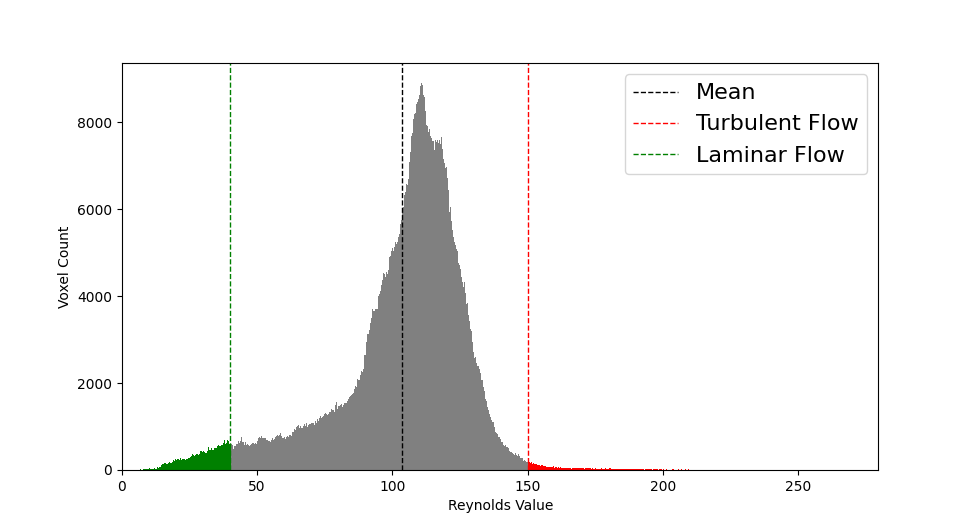
\includegraphics[scale=.35]{Figures/Hist4_11.png}
\decoRule
\caption[Reynolds Number Histogram]{Mean Reynolds Values Histogram}
\label{fig:MHistgram}
\end{figure}

\begin{figure}
\centering
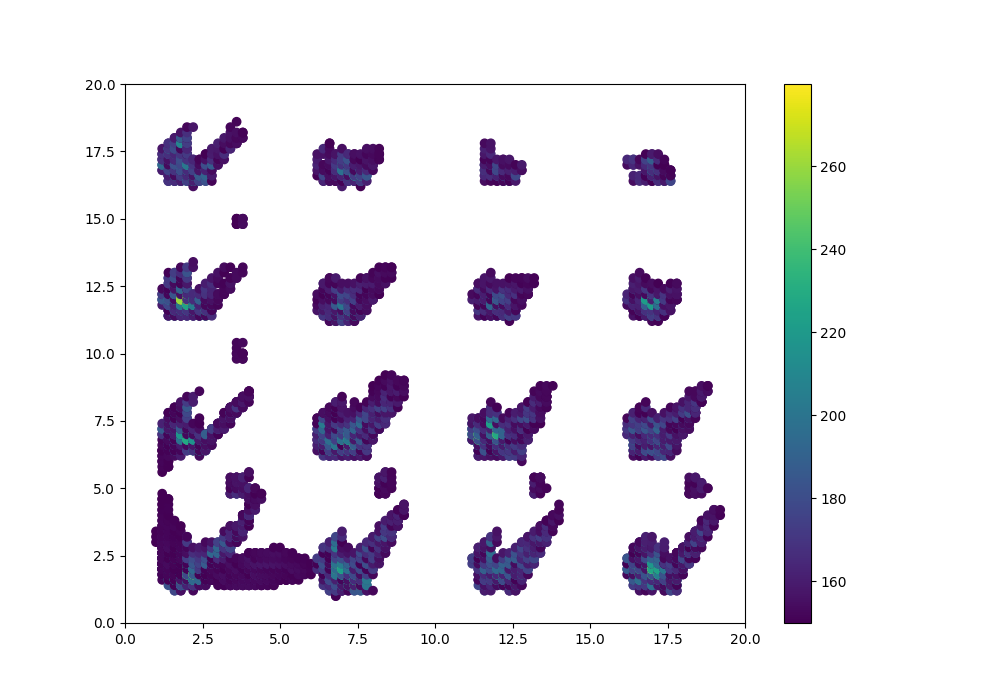
\includegraphics[scale=.35]{Figures/Turb2D_4_11.png}
\decoRule
\caption[Turbulent Air Flow Scatter Plot]{A top down view of a plot showing areas of turbulent air flow containing 7705 points}
\label{fig:MTurbulentflow}
\end{figure}
%-----------------------------------
%	SECTION 2
%-----------------------------------
\section{Pathline Calculations}


Now that we have calculated these points of interest we can use an Ordinary Differential Equation solver to calculate the streamlines. We will use a fifth-order Runge-Kutta method for adaptive time steps and to minimize errors in calculations. We are able to use forward and reverse integration to calculate path lines for every time step that passes through these points of interest. After integrating in both directions we then combine the posting and time data for each pathline while also adding in the Reynolds Number for each point as well. We store all of this data in hdf5 files so it can be efficiently loaded into our visualization pipeline. 


%-----------------------------------
%	SECTION 3
%-----------------------------------
\section{Unity Visualization}
Once we read in pathline and scene data into Unity,
we determine the largest (\ensuremath{RE_{max}}) and smallest (\ensuremath{RE_{min}}) value within the data set.  Now having the minimum and maximum values we are  able to calculate a color value for each segment of the pathlines. To do so we have to calculate the interpolant value within the range [\ensuremath{RE_{min}}, \ensuremath{RE_{max}}] (Eqn. \ref{eq:3}). This provides us with a value between [0,1] and then we can map this value to a color on a perceptually uniform color map \color{red} [We use  vega's magma color map with 8 colors] \color{black} For each time step we load in the respective data for all \ensuremath{k} pathlines. To resolve the issue of being able to see orientation but not true directionality of a pathline (a line going left to right looks identical to a line going right to left) we segment each pathline into n-1 line segments  (e.g. \ensuremath{P_0\rightarrow P_1},\ensuremath{P_1 \rightarrow P_2},...,\ensuremath{P_{n-2} \rightarrow P_{n-1}}).
We then adjust the starting width of each line segment to be the average length of a voxel and the ending width zero. Figure \ref{fig:UnityPathline} illustrates the benefits of this visual change. Using cones resolves the issues with direction of pathlines as previously discussed. We then build a color gradient texture and apply it to the texture from point to point with the precalculated color map. We are able to compile and build our Unity system into an executable file that allows for the end user to run on any compatible system. We have the user interface (UI) designed to allow for viewing the simulation using a Head Mounted Display (HMD), a virtual reality headset, and controller or a computer monitor with a keyboard and mouse for movement. Users just need to  type in the directory of the hdf5 files output discussed previously and the data is cached for quick loading into the simulation. users are then able to move around  the environment in either Virtual Reality or just by using the mouse and keyboard. 

\begin{equation} \label{eq:3}
f(RE_{min},RE_{max},RE_{value}) = \frac{RE_{value}-RE_{min}}{RE_{max}-RE_{min}}
\end{equation} 

\begin{figure}
\centering
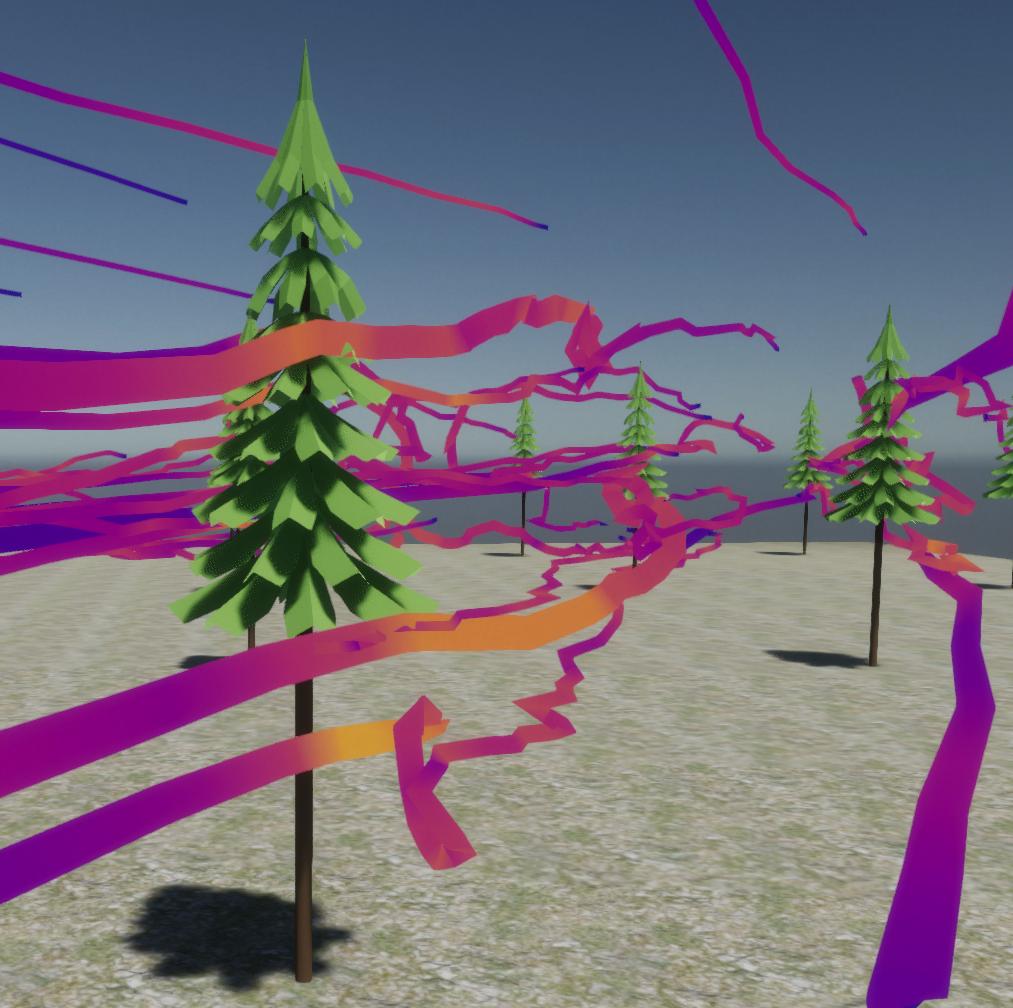
\includegraphics[scale=.3]{Figures/TreePathline1.png}
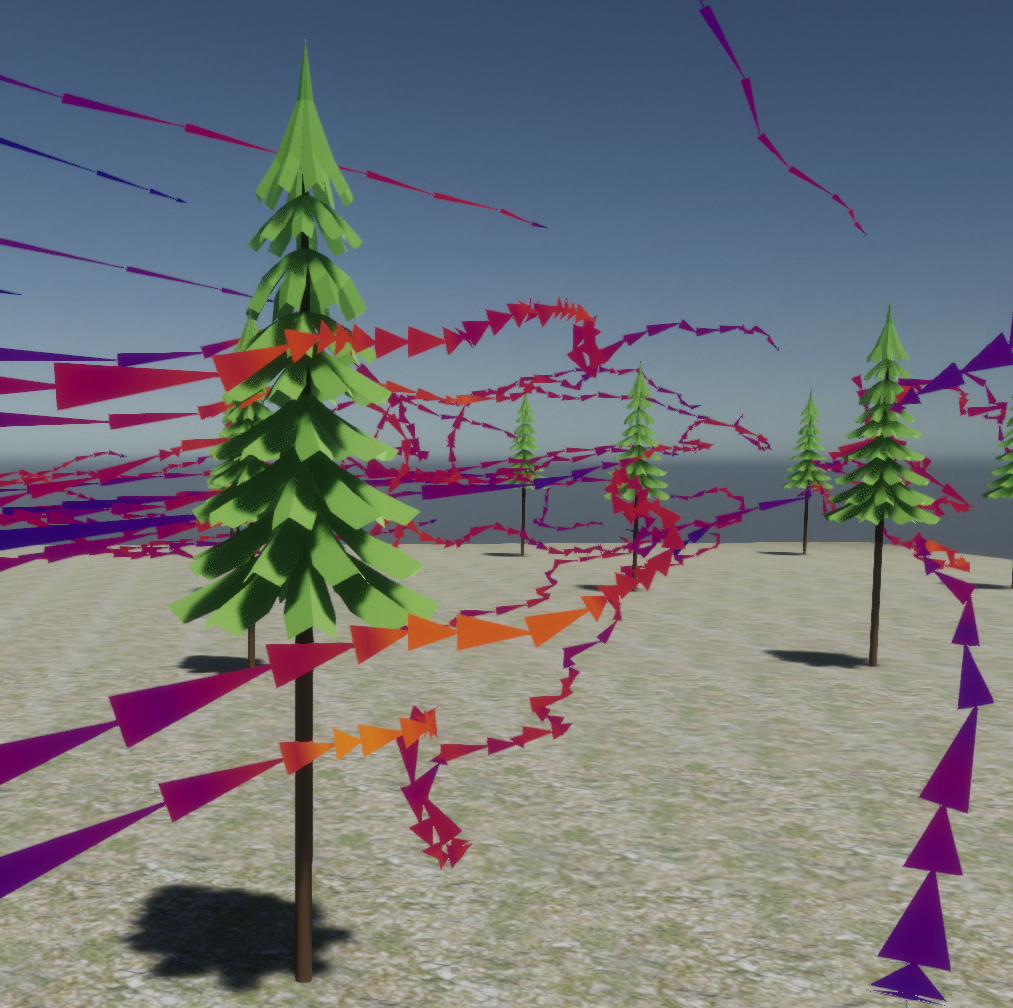
\includegraphics[scale=.3]{Figures/TreePathline2.png}
\decoRule
\caption[Pathlines comparisons in Unity]{\textbf{Top:} Pathlines visualized as a single line  \textbf{Bottom:} Pathlines broken in to line segments }
\label{fig:UnityPathline}
\end{figure}
 
% Chapter Template

\chapter{Results} % Main chapter title

\label{Chapter3} % Change X to a consecutive number; for referencing this chapter elsewhere, use \ref{ChapterX}

%----------------------------------------------------------------------------------------
%	SECTION 1
%----------------------------------------------------------------------------------------
\section{Setup}
In this paper, we discussed a pipeline implemented using python then with C\# and Unity's real time development platform as the visualization engine. We ran a Levelset 4, FDS simulation, set to output plot3D every 0.5 seconds on a 20m x 20m x 20m mesh, containing voxels  0.2m x 0.2m x 0.2m  in size, with open boundary conditions. The simulation was 100 seconds in length with a ground fire igniting 10 seconds in to the simulation, with a wind of 5.6 m/s originating from the south west (215\textdegree) and trees evenly distributed on the mesh. [Figure \ref{fig:CFDTopDown} shows a top down view of our visualization rendered in SmokeView] \par
[Github link to fds file?]\par
\section{Analyses}
The total run time for this simulation was  \color{red}252 (4 Hours 12 Min ) \color{black} minutes to complete, running 4 cores of an i7 4790k in parallel, while calculations we disused in this paper were able to complete in \color{red} 3 \color{black} minutes, with no parallelization at the moment. Additionally, the size of the CFD output files was 5.0 GB while the saved data needed for full Virtual Reality using our methodology is 28.9 MB a 99.4\% reduction in file size. The use of unity's development platform allows us to compile and the possibility to make available for distribution a self-contained system to help improve training for fire fighters.


\begin{figure}
\centering
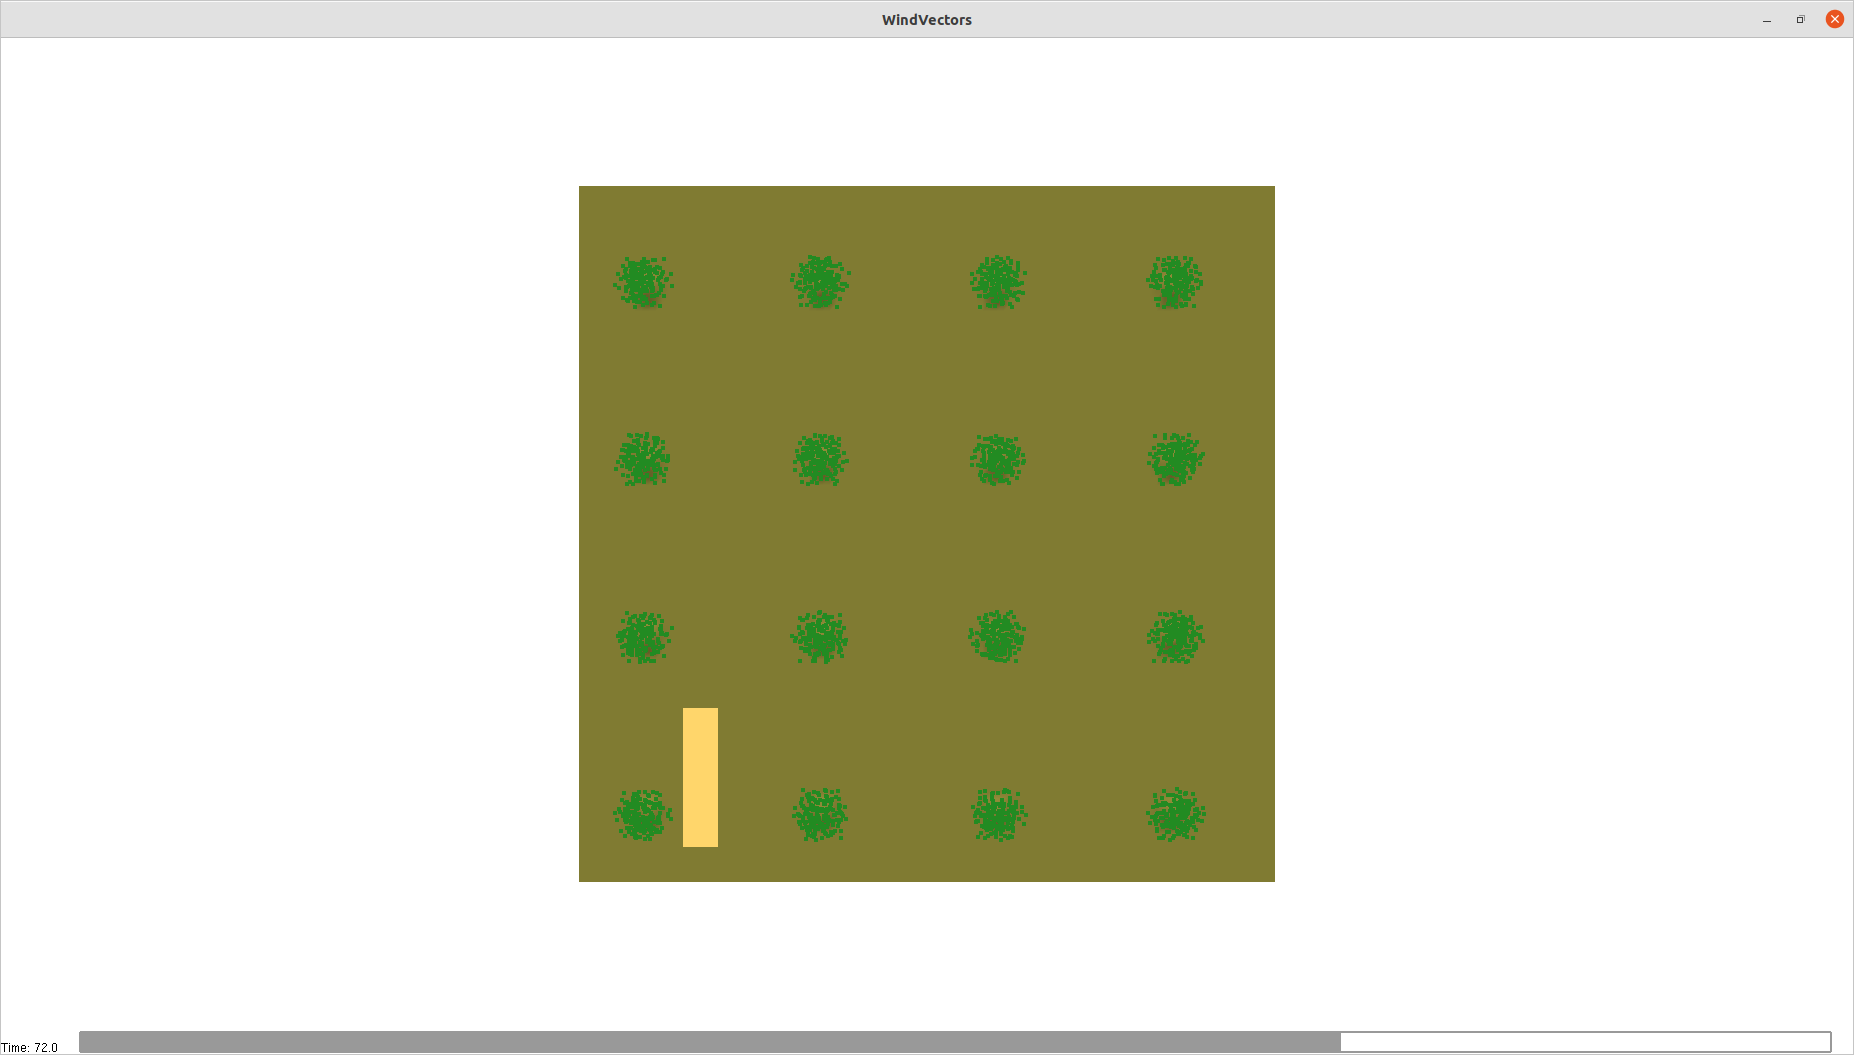
\includegraphics[scale=.1]{Figures/fdsPartTopView.png}
\decoRule
\caption[CFD Simulation]{A top-down view of the CFD simulation}
\label{fig:CFDTopDown}
\end{figure}
% Chapter Template

\chapter{Conclusion and Future Work} % Main chapter title

\label{Chapter4} % Change X to a consecutive number; for referencing this chapter elsewhere, use \ref{ChapterX}

Updating the tools available for fire fighter training is a current point of interest for the forestry service. It also has the capability to save life's if done effectively. Our goal with this project was to design a generalized proof of concept that would be able to be built on to improve training and safety for firefighters. \par
We were able to show with trivial increase to the amount of time for the current pipeline of running and visualizing a simulation, we were able to substantial lower the total about of memory needed to store pertinent data to be visualized. While also improving the fidelity of the visualization we are able to allow firefighters to experience simulations without the risks of a real fire. This allows for each user to have a larger mental set of fire environments they have experienced before being put in a dangerous situation, witch will allow them to make more accurate assessments of real life situations and be safer overall. \par

In the future further research in to improving or implementing new thresholding and clustering techniques might have the capability to further optimize our pipeline. As for future capabilities for unity implementation of additional libraries to allow for these projects to run on the Oculis platform would lower the cost of equipment needed for each training facility, additionally further research in to utilizing Unitys WebVR would allow for the system to be hosted online and accessed remotely again lowing the total cost of the equipment needed for each training facility  

 
%\include{Chapters/Chapter5} 

%----------------------------------------------------------------------------------------
%	THESIS CONTENT - APPENDICES
%----------------------------------------------------------------------------------------

\appendix % Cue to tell LaTeX that the following "chapters" are Appendices

% Include the appendices of the thesis as separate files from the Appendices folder
% Uncomment the lines as you write the Appendices

%% Appendix A

\chapter{Frequently Asked Questions} % Main appendix title

\label{AppendixA} % For referencing this appendix elsewhere, use \ref{AppendixA}

\section{How do I change the colors of links?}

The color of links can be changed to your liking using:

{\small\verb!\hypersetup{urlcolor=red}!}, or

{\small\verb!\hypersetup{citecolor=green}!}, or

{\small\verb!\hypersetup{allcolor=blue}!}.

\noindent If you want to completely hide the links, you can use:

{\small\verb!\hypersetup{allcolors=.}!}, or even better: 

{\small\verb!\hypersetup{hidelinks}!}.

\noindent If you want to have obvious links in the PDF but not the printed text, use:

{\small\verb!\hypersetup{colorlinks=false}!}.

%\include{Appendices/AppendixB}
%\include{Appendices/AppendixC}

%----------------------------------------------------------------------------------------
%	BIBLIOGRAPHY
%----------------------------------------------------------------------------------------

\printbibliography[heading=bibintoc]

%----------------------------------------------------------------------------------------

\end{document}  
